\chapter{Implementación}

\section{Configuración del entorno en NetBeans 12}

El proceo de configuración del entorno en la plataforma de desarrollo NetBeans 12, la cual también usamos durante el desarrollo de la asignatura Desarrollo Basado en Agentes, fue cuanto menos tedioso. Todo el conglomerado de proyectos que posibilitan la ejecución de LATEN es necesario configurarlo, idealmente, a la vez y de manera uniforme.\\

Los diferentes proyetos fueron proporcionados por el tutor del proyecto de manera gradual, para de igual forma intentar acoplarlos al nuevo proyecto que se creó, perteneciente al propio agente LATEN. Esto en un primer momento ocasionó problemas de dependencias, tanto de proyectos como de archivos Java \textit{(con terminación .jar)}, incluso de otros paquetes de apoyo.\\

No obstante, tras unas horas de trabajo conjunto con el tutor, se pudo configurar de manera absoluta el proyecto LATEN.\\

Los proyectos de NetBeans de los que depende LATEN de una manera u otra, se listan a continuación:

\begin{itemize}
	\item BaseTelegram
	\item CoreLARVAAdminObjects
	\item CoreLARVAAgents
	\item CoreLARVAObjects
	\item CoreLARVAMoreObjects
	\item PTelegram
\end{itemize}

Adicionalmente, se requieren también los siguientes archivos con terminación \textit{.jar}:

\begin{itemize}
	\item Conector Java-MySQL, versión 8.0.25
	\item JADE
	\item La librería de utilidades Commons IO
\end{itemize}

Es importante mencionar también que se requiere de la versión 11 de JDK \textit{(\textbf{J}ava \textbf{D}evelopment \textbf{K}it)} para el correcto funcionamiento de todos los proyectos.\\

Una vez se tienen todos los proyectos correctamente importados, y las librerías debidamente incorportadas, se puede proceder con el resto de configuraciones necesarias antes de poder empezar con la implementación de nuestro agente.

\section{Configuración de la base de datos}

Con respecto a la configuración de la base de datos, el profesor de la asignatura me proporcionó un script SQL para poder tener una copia local de la base de datos tal y como se había usado para la asignatura. En dicha copia de la base de datos, se eliminaron aquellos datos de carácter sensible de otros alumnos que no influirían posteriormente en el propio proyecto, como por ejemplo el correo electrónico institucional de la Universidad de Granada o el número de identificación del chat personal de Telegram de cada alumno.\\

Para la gestión de la base de datos es buena práctica usar un cliente, ya sea web o con aplicación nativa, ya que permite una mejor visualización de toda la estructura de la base de datos, así como de los propios datos que alberga. Es evidente que también se puede usar la terminal de, en mi caso, el sistema operativo Ubuntu 20.04, para llevar a cabo todas las labores de gestión de la base de datos.\\

En mi caso, por preferencias personales, decidí instalar el gestor \textbf{phpMyAdmin}, el cual es una interfaz gráfica de usuario disponible a través de web, accediendo desde la dirección \textit{http://localhost/phpmyadmin}.\\

Para la instalación de dicho cliente desde la terminal de Ubuntu 20.04, se deben seguir unos pasos concretos. En primer lugar, se debe ejecutar el comando

\begin{lstlisting}
    sudo apt update
\end{lstlisting}

para actualizar la lista de paquetes disponibles y sus versiones. A continuación, el comando para proceder a la instalación del paquete de phpMyAdmin, así como de sus dependencias es el siguiente:

\begin{lstlisting}
    sudo apt install phpmyadmin php-mbstring php-gettext
\end{lstlisting}

Este comando, al ejecutarlo, nos ofrecerá una interfaz gráfica para especificar ciertos parámetros de configuración para el cliente. Entre ellos, deberemos establecer las contraseñas del usuario administrador de la base de datos, así como de la propia aplicación MySQL. Además, deberemos de seleccionar en qué servidor web queremos que se ejecute phpMyAdmin: \textit{apache2} o \textit{lighttpd}. Escogí \textit{apache2} por estar más familiarizado con el mismo.\\

Una vez completado el proceso de instalación mediante la terminal, ya podremos acceder a la interfaz gráfica a través del enlace anteriormente mencionado: \textit{http://localhost/phpmyadmin}.\\

El siguiente paso, será importar el script SQL que facilitó el tutor de la asignatura. Desde la interfaz gráfica, primeramente deberemos crear la base de datos en la que posteriormente importaremos dicho script. A la base de datos, le otorgué el nombre \textbf{LATEN}. Se puede crear una base de datos de manera muy sencilla como se muestra en la figura \ref{img:menubd1}. Basta con introducir el nombre de la base de datos que queremos crear y posteriormente pulsar sobre el botón \textbf{Crear}.

\begin{figure}[h]
\centering
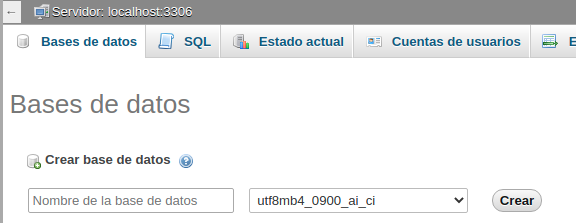
\includegraphics[width=0.9\textwidth]{logos/menubd1.png}\\[1.4cm]
\caption{Pestaña de creación de base de datos en phpMyAdmin}
\label{img:menubd1}
\end{figure}

Una vez creada la base de datos, navegaremos hacia ella a través de la interfaz gráfica y pulsaremos sobre el botón \textbf{Importar} del menú superior de phpMyAdmin. En esta ventana, podremos importar fácilmente el archivo con extensión \textit{.sql} aportado por el tutor de la asignatura, como se muestra en la figura \ref{img:menubd2}. Una vez cargado el script, presionaremos sobre el botón \textbf{Continuar} situado al pie de dicha página, y acto seguido tendremos disponible nuestra base de datos, con todas las tablas y con todos los datos correspondientes.

\begin{figure}[h]
\centering
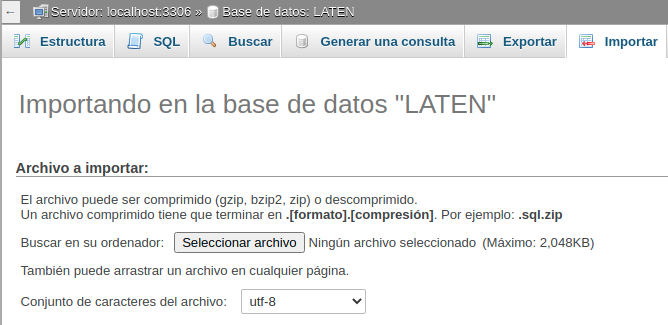
\includegraphics[width=0.9\textwidth]{logos/menubd2.png}\\[1.4cm]
\caption{Pestaña de importación en phpMyAdmin}
\label{img:menubd2}
\end{figure}


\section{Configuración y entorno de JADE}

Como se explicó en la sección \ref{sec:jade}, JADE es un framework que actuará de middleware entre nuestro sistema de agentes.\\

Su configuración es bastante sencilla. En la ya mencionada asignatura, se nos proporcionó un fichero comprimido que contiene todo lo necesario para la instalación de JADE. Con la siguiente secuencia de comandos, instalaremos de manera muy sencilla el paquete:

\begin{lstlisting}
    unzip dba-jade-kit.zip
    cd bin
    sudo ./install.sh
\end{lstlisting}

Una vez instalado, podemos ejecutar el servicio de JADE haciendo uso del siguiente comando:

\begin{lstlisting}
    sudo ./doJade.sh start
\end{lstlisting}

y de igual forma, cambiando el argumento, para detener el servicio:

\begin{lstlisting}
    sudo ./doJade.sh stop
\end{lstlisting}

Estas herramientas que acabamos de instalar también gozan de una interfaz gráfica desde la que observar todos los agentes que se encuentran disponibles en la plataforma además de las comunicaciones que se realizan entre ellos. Para ejecutar dicha interfaz gráfica, usaremos el siguiente comando:

\begin{lstlisting}
    sudo ./doJadeGUI.sh 
\end{lstlisting}

El cual, tras unos instantes nos mostrará una pantalla como la que se muestra en la figura \ref{img:jade1}.

\begin{figure}[h]
\centering
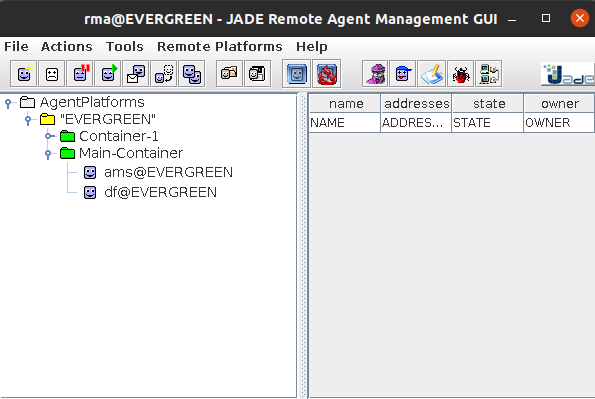
\includegraphics[width=0.9\textwidth]{logos/jade1.png}\\[1.4cm]
\caption{Interfaz gráfica de JADE}
\label{img:jade1}
\end{figure}

\section{Configuración del agente}

Para que nuestro agente se integre de manera correcta en la red con el resto de agentes que ya habitan en ella, es necesario especificar ciertos parámetros de configuración que posteriormente serán leídos por las clases correspondientes que lanzan dicho agente a la plataforma JADE. Estos parámetros de configuración se establecerán en formato JSON, dentro de una carpeta llamada \textit{config} del mismo proyecto de nuestro agente LATEN.\\

Dichos parámetros de configuración son los que se muestran a continuación:

\begin{lstlisting}
    {
        "name": "LATEN",
        "version": "1.0",
        "silent": false,
        "log": true,
        "system": true,
        "showbehaviour": false,
        "singlebehaviour": true,
        "boot": "jade",
        "jadeconnection": {
            "host": "localhost",
            "port": 1099
        },
        "dbconnection": {
            "host": "localhost",
            "port": 3306,
            "database": "LATEN",
            "user": "username",
            "password": "password"
        }
    }
\end{lstlisting}

A destacar de este archivo de configuración, podemos ver el elemento \textbf{singlebehaviour}, el cual tiene como valor asignado \textit{true}, lo cual indica que dicho agente tiene un solo comportamiento y por tanto no es necesario establecer configuraciones adicionales a la hora de lanzar dicho agente, como por ejemplo sería establecer un sistema de colas múltiple para la recepción de mensajes ACL.\\

Otros elementos como \textbf{silent}, \textbf{log} o \textbf{system}, tienen como propósito informar al desarrollador sobre los distintos acontecimientos durante la ejecución de dicho agente. Se pueden configurar a \textbf{true} o \textbf{false} para ajustar la cantidad de información que queremos recibir de la ejecución.\\

Adicionalmente, tenemos un elemento de configuración de la conexión de JADE llamado \textbf{jadeconnection}, en el que podemos especificar el \textbf{host} y el \textbf{puerto \textit{(port)}} a través de los cuales se puede establecer una conexión con JADE.\\

Por último, tenemos el elemento \textbf{dbconnection} que posee toda la configuración necesaria para establecer conexión con la base de datos previamente configurada.

\section{Implementación}

\subsection{Comunicación con el agente LATEN}